\section{Background}
\subsection{LLM Generative Tasks}
\label{sec:llmdecoding}

\begin{figure}[!t]
    \centering    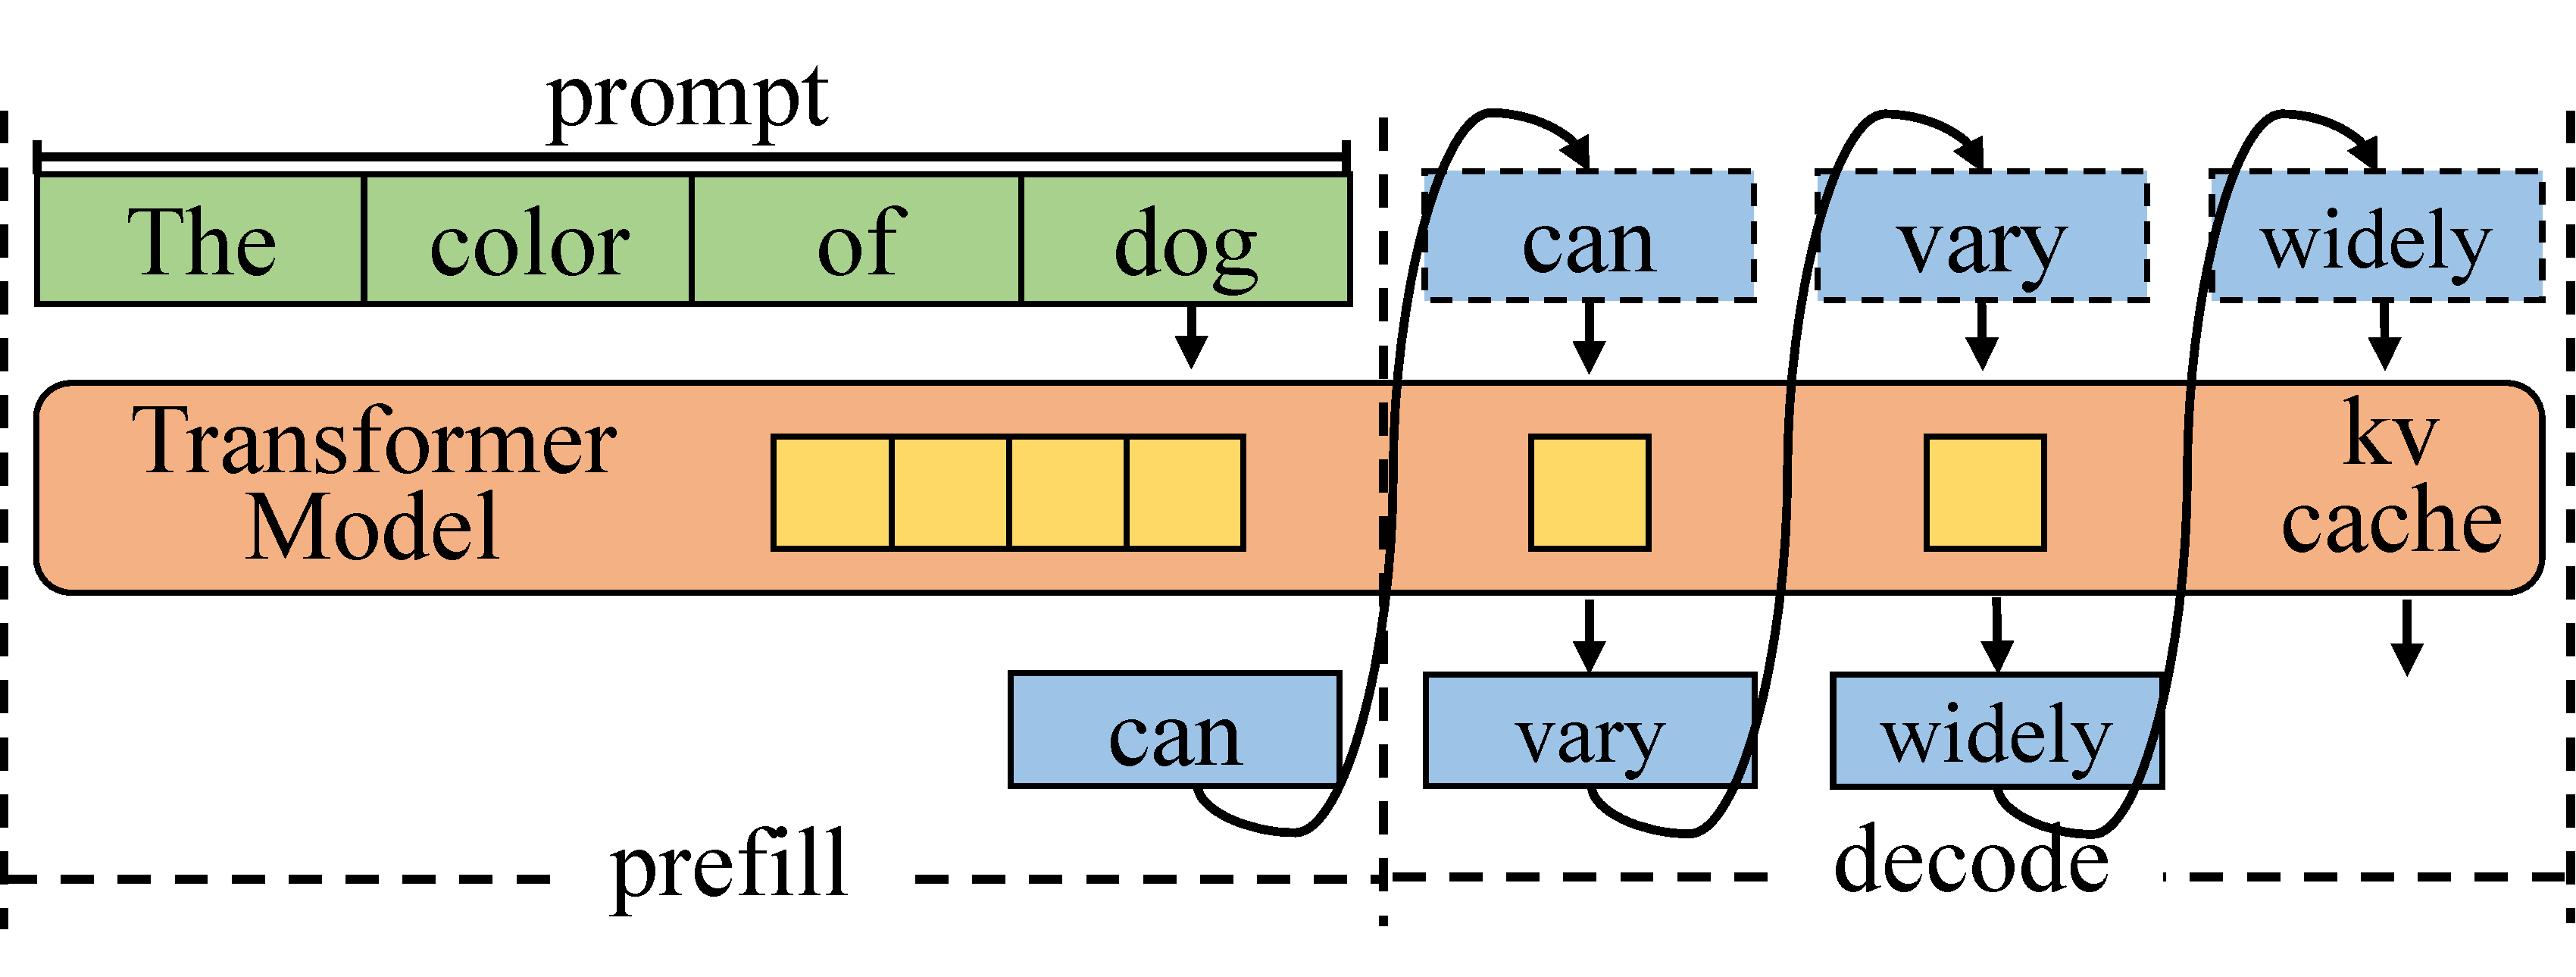
\includegraphics[width=0.75\linewidth]{fig/gen-task.pdf}
    \caption{The generate process of LLM generative task.}
    \label{fig:gen-task}
    \vspace{-8pt}
\end{figure}
Modern LLM generative tasks follow the autoregressive decoding process and predict the next token given an input sequence.
During this, intermediate states, known as KV cache, are generated at each token position.
Through maintaining KV cache in memory, the modern LLM inference systems can eliminate most redundant computation in this iterative process.
Based on whether the KV cache has been generated, the inference process is divided into prefill and decode phases.
As illustrated in Figure~\ref{fig:gen-task}, the prefill phase deals with the newly-incoming prompt (in green) and initializes the KV cache (in gold), often comprising many tokens, and processes these tokens concurrently to generate a new token (in blue).
Next, benefiting from KV cache, each step of the decode phase only processes one new token from the previous step. LLM generative tasks have some key features:
\begin{itemize}[leftmargin=*]
    \item First, the prefill and decode have significant computational differences. For the prefill, it processes many tokens in parallel and easily becomes compute-bound. In contrast, the decode is more constrained by the memory bandwidth for it has a similar amount of I/O and only processes a single token for a single request. Thus, a very small batch size is sufficient for the prefill phase to saturate computational resources, while the decode phase requires a substantially larger batch size.
    \item Second, inherent uncertainty arises from the variable-length nature. Both input and output lengths vary, and the output length typically remains unknown until inference completes.
\end{itemize}

\subsection{Opportunities of Pipeline Parallelism for High-Throughput LLM Inference}

\subsubsection{High-Throughput LLM inference}

 
While online LLM serving has garnered significant attention, scenarios without strict latency constraints, such as the RLHF rollout stage~\cite{hu2024openrlhfeasytousescalablehighperformance} and data augmentation for recommendation systems~\cite{ding-etal-2024-data}, are also important for modern intelligent applications.
In such scenarios, pursuing high throughput becomes the top priority. 
\begin{figure}[t]
    \centering    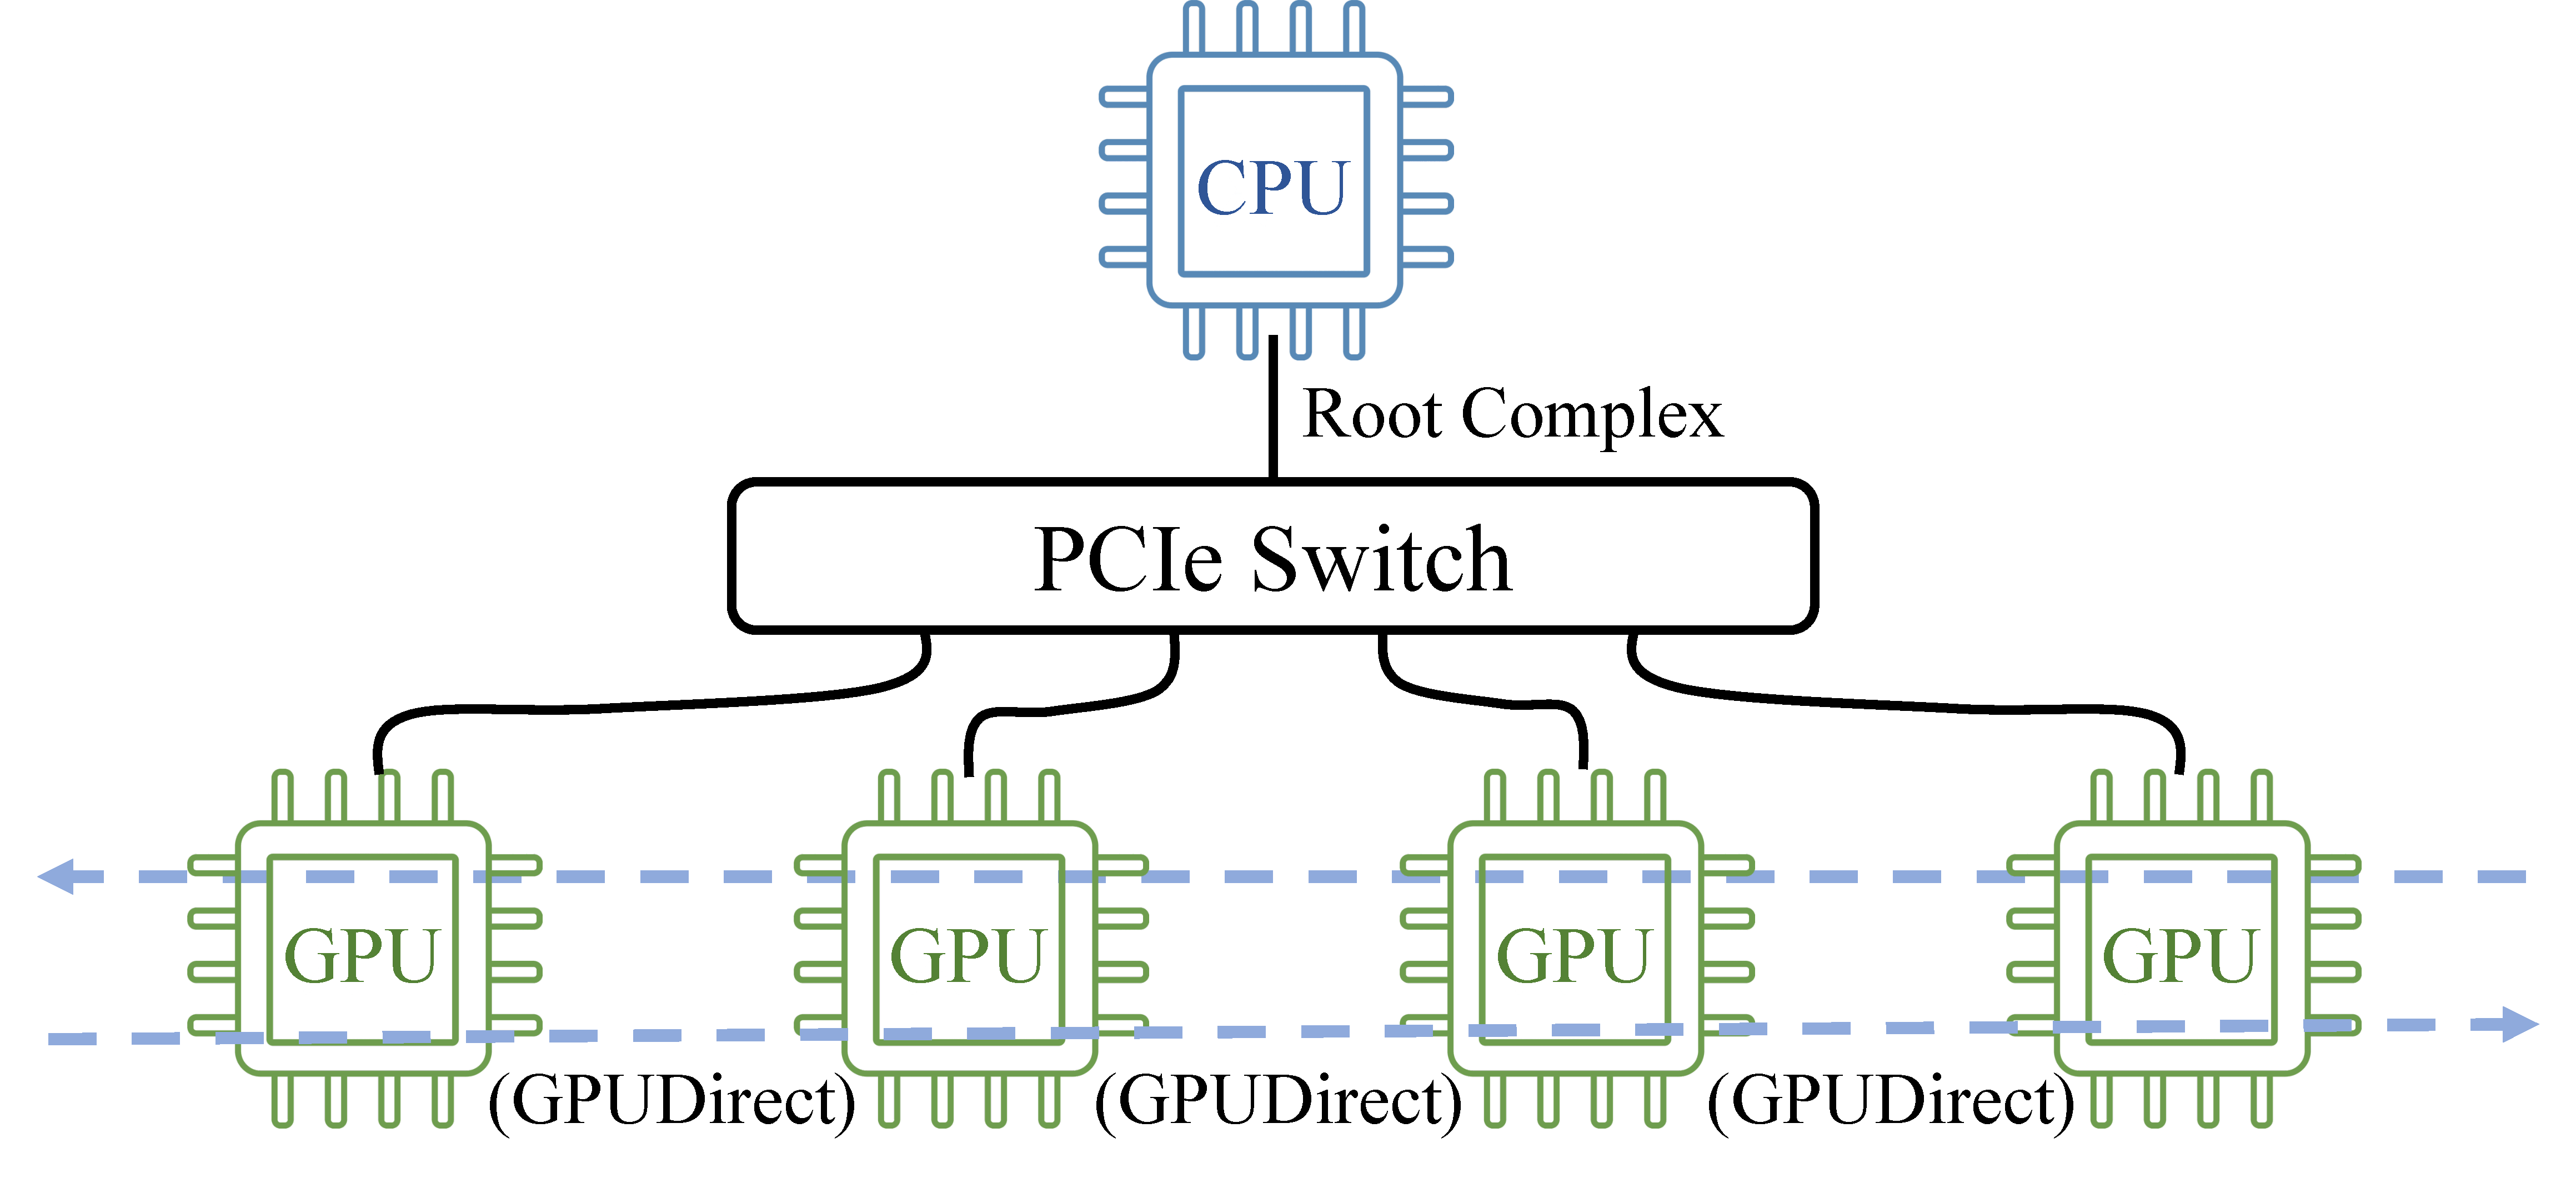
\includegraphics[width=0.75\linewidth]{fig/multigpu.pdf}
    \caption{The multi-GPU architecture.}
    \label{fig:multigpu}
\end{figure}

First, achieving high-throughput LLM inference requires sufficient memory capacity.
During inference, both model weights and KV cache demand substantial memory.
Commonly-used LLMs have 7B, 13B, 30B, 70B, or even more weights, exceeding the memory capacity of most devices, especially these commodity devices such as NVIDIA A10 (24GB), 4090 (24GB), and L20 (48GB).
In addition to weights, hundreds of requests should coexist in the decode phase for saturating GPU resources and KV cache contributes significantly to memory usage. 
For example, the KV cache of a single token in the Llama-30B~\cite{touvron2023llama} occupies 1.52 MB, and 400 requests with an average length of 300 would require approximately 178 GB of memory. 

Second, achieving high-throughput LLM inference requires minimizing coordination overhead when utilizing multiple resources to expand memory capacity.
Figure~\ref{fig:multigpu} illustrates the popular multi-GPU architecture widely used in deploying LLMs, where multiple GPUs connect to a single CPU.
Under this architecture, there are typically two major approaches to improve memory capacity: offloading and parallelization.


\begin{figure}[!t]
    \centering    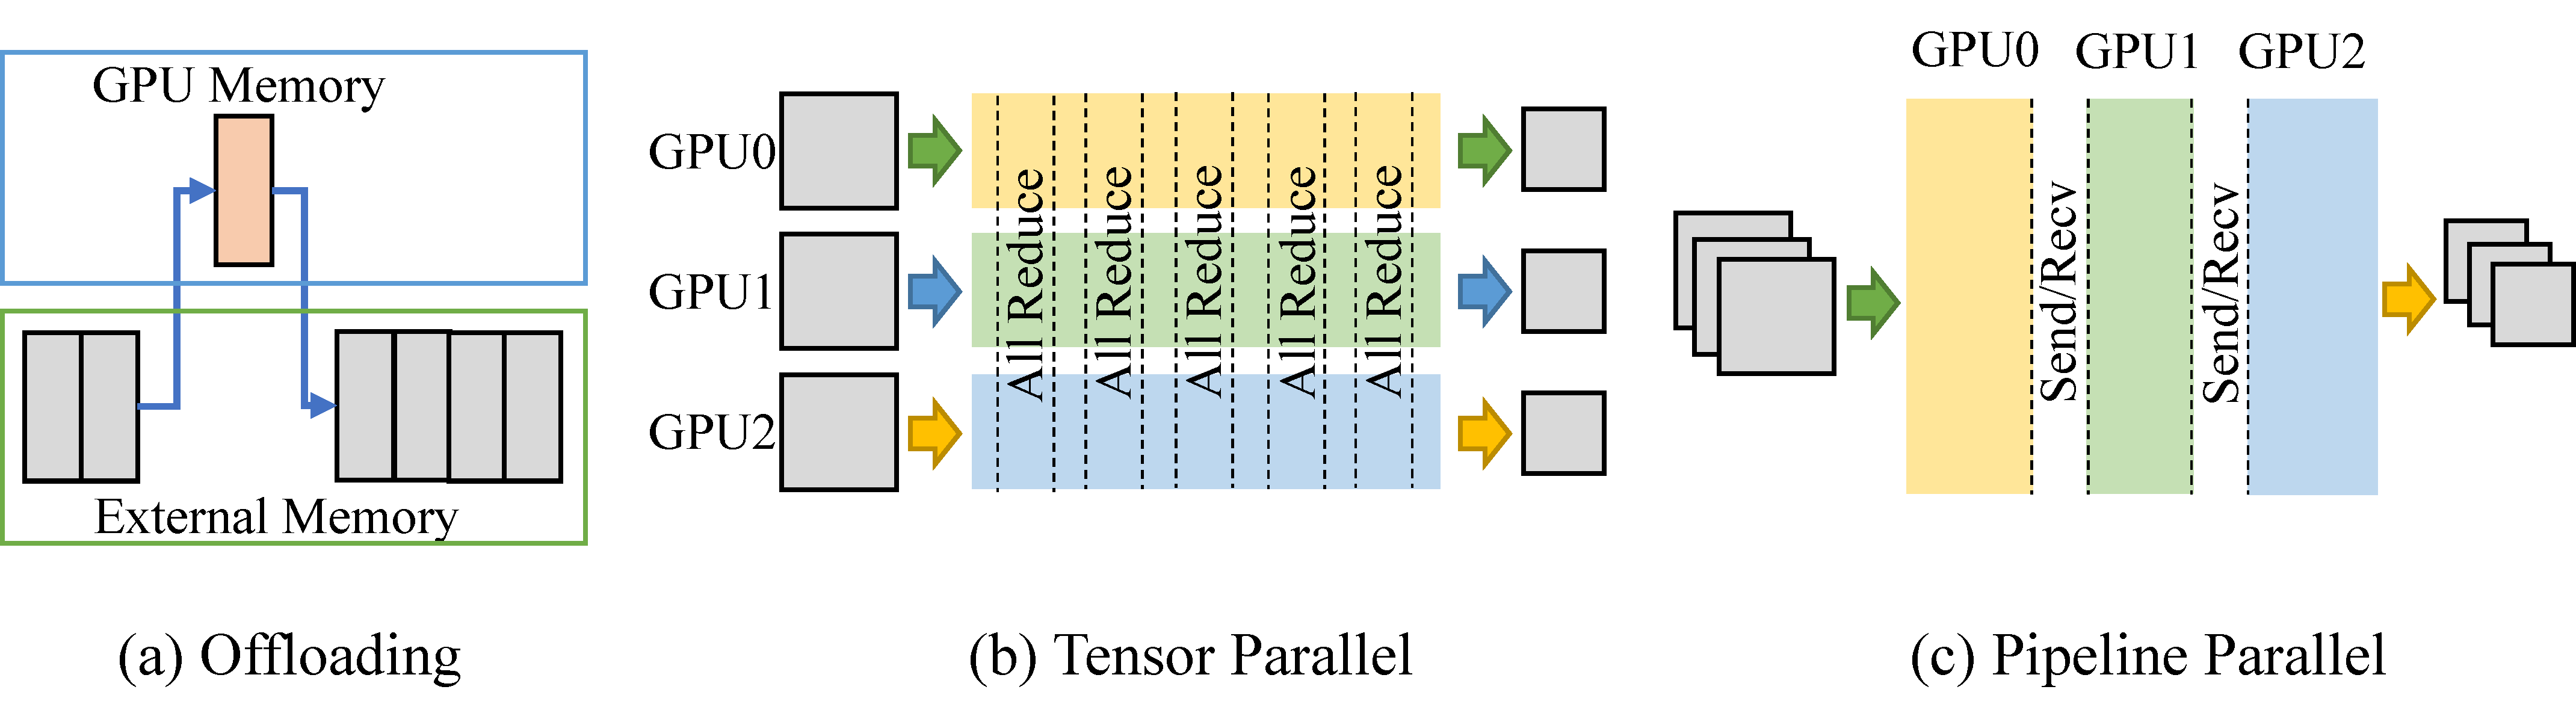
\includegraphics[width=0.95\linewidth]{fig/moremem.pdf}
    \caption{Offloading and parallel approaches.}
    \label{fig:moremem}
\end{figure}

\subsubsection{Coordination Overhead in Offloading Approach}

As shown in Figure~\ref{fig:moremem}(a), a single inference instance can acquire more memory capacity through offloading data to secondary storage.
Through iteratively exchanging data between host memory and GPU memory, this allows the decode phase to accommodate more requests for processing at a given moment.
However, the PCIe bandwidth can be the bottleneck for this approach even when the CPU-to-GPU ratio is 1:1.
It encounters more severe PCIe contention in a multi-GPU architecture when multiple GPUs simultaneously offload data to host memory.
In other words, the substantial coordination overhead between CPU and GPU makes this approach infeasible for high-throughput LLM inference.

\subsubsection{Coordination Overhead in Parallel Approaches}

\begin{figure}[!t]
    \centering    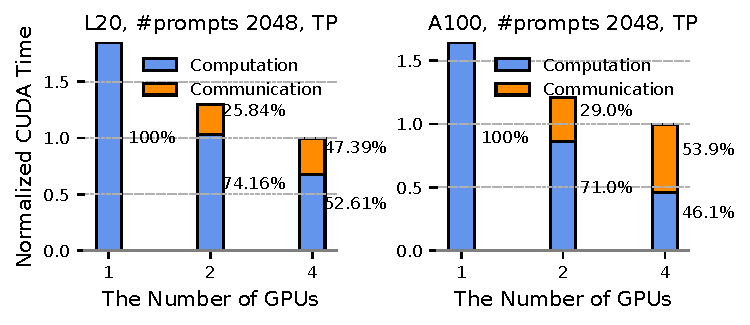
\includegraphics[width=0.95\linewidth]{graph/background_TD_Pipe.pdf}
    \caption{Execution time breakdown of the prefill phase using the tensor parallel approach in a multi-GPU architecture.}
    \label{fig:background_TD}
\end{figure}

Through distributing LLMs to multiple devices, an instance can acquire more memory capacity.
Figure~\ref{fig:moremem}(b) and (c) show the tensor parallel (TP) and pipeline parallel (PP) approaches.
TP shards each layer across multiple GPUs, with the model weights and KV cache being equally distributed across GPU workers.
It demands frequent communications that a single Transformer layer necessitates two rounds of all-reduce operations.
We deliver distributed inference case studies of Llama-30B~\cite{touvron2023llama} on two nodes without direct cables in FP16.
To demonstrate strong scalability, we reduce the number of layers in the model to fit into fewer devices and report the running results, shown in Figure~\ref{fig:background_TD}.
Notably, the model is composed of layers with the same structure, so reducing the number of layers does not affect its computational or communication characteristics.

The overall execution time on the L20 node is reduced by 1.84$\times$ when increasing the number of devices from 1 to 4.
Despite the reduction in total execution time, communication time accounts for 47.39\% of the total time on 4 devices.
On the A100 node, the overall execution time is only reduced by 1.64$\times$, with communication time consuming up to 53.9\% of the total time on 4 devices.
Thus, the tensor parallel approach heavily relies on interconnection capability and leaves computational resource idle for long period. 
Furthermore, certain high-performance GPUs enable direct communication through specialized cables, like NVIDIA's NVLINK, which significantly enhances their communication efficiency but also largely raises the node price.

Compared to TP, PP splits a model layer-wise, where each device is responsible for a subset of layers. 
It only requires a single point-to-point communication with a much smaller data volume every few layers.
Although the imbalanced pipeline workloads and complex data dependencies of LLM inference still prevent it from being the primary choice in the latency-sensitive scenarios,  the largely-reduced communication makes PP a promising approach to support throughput oriented LLM inference, especially on commodity hardware that high-performance connectivity like NVLINK is unavailable.

\subsection{Existing Pipeline Parallelism for LLM Inference}
\label{sec:batching}
Existing pipeline parallelism mainly differs in batching approaches.
To fully utilize modern GPUs, the batching technique is commonly adopted for processing deep learning workloads, where multiple samples are processed simultaneously to expose high parallelism and provide considerable hardware performance improvements.
There are mainly separate batching and hybrid batching for LLMs.

Separate batching schedules requests exclusively for the prefill phase or exclusively for the decode phase, without mixing them in the same batch. Given that these two phases exhibit distinct performance characteristics, i.e. compute-bound and memory-bound, the prefill phase saturates GPU computation even at a batch size of just one, while the decode phase requires a batch size in hundreds.
At each time, the inference instance will stay either in the prefill phase or in the decode phase.
By contrast, hybrid batching combines requests from both the prefill and decode phases into the same batch, forming hybrid batches.

When integrated with pipeline parallelism, these two batching approaches exhibit distinct advantages and disadvantages, yet both continue to suffer from severe pipeline bubble issues.
With separate batching, it is straightforward to manage batches consisting solely of prefill-phase requests, which can be launched continuously since there are no inter-batch data dependencies. Similarly, decode-only batches are convenient for achieving inter-batch load balance, as each decode step processes a single token with relatively uniform workload. However, mixing prefill and decode requests within the same batch introduces data dependencies and workload imbalance, which can lead to severe pipeline bubbles.
Moving to hybrid batching, it is typically integrated with the chunked prefill approach~\cite{agrawal2024taming}, which splits the prefill into chunks and enables to achieve better inter-batch load balance.
However, 1) as decode steps are added to all batches, it becomes essential to manage data dependencies across all batches, 2) the highly variable input and output lengths still lead to severe load imbalance, 3) Moreover, chunked prefill introduces repeated KV cache access as overhead.
